
In this section, we introduce our representation of 3D traffic participants and our modeling of object-object occlusion relationships. We refer the reader to Figure~\ref{fig:reflectiontransimission} for an illustration of the proposed concepts.

\begin{figure}
  \usetikzlibrary{calc}
  \centering
  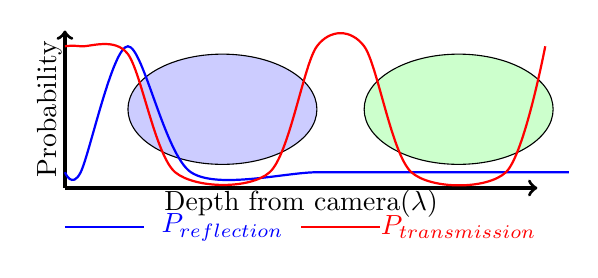
\begin{tikzpicture}
         \path [fill=blue!20,draw] (0,0) ellipse (1.2 and 0.7);
     \path [fill=green!20,draw] (3,0) ellipse (1.2 and 0.7);
     \coordinate (o) at (-2,-1);
     \draw(o) edge [->,very thick] node (xa) {} +(6, 0);
     \node at ($(xa) + (0, -0.2)$) {Depth from camera($\lambda$)};
     \draw(o) edge [->,very thick] node (ya) {} +(0, 2);
     \node [rotate=90]at ($(ya) + (-0.2, 0)$) {Probability};
    \draw [thick,blue]plot [smooth] coordinates {($(o)+(0,0.2)$) ($(o)+(0.2,0.2)$) ($(o) + (0.8, 1.8)$) ($(o)+(1.6,0.2)$) ($(o)+(3.2,0.2)$) 
      %($(o)+(3.8,1.8)$)  % Transmission prob corresponds to particular object
    ($(o)+(4.4,0.2)$) ($(o)+(6.4,0.2)$) };
    \draw [thick,red] plot [smooth] coordinates {($(o)+(0,1.8)$) ($(o)+(0.2,1.8)$) ($(o) + (0.8, 1.7)$) ($(o)+(1.4,0.2)$) ($(o)+(2.6,0.2)$) ($(o)+(3.2,1.8)$) ($(o)+(3.8,1.8)$) ($(o)+(4.4,0.2)$) ($(o)+(5.6,0.2)$) ($(o)+(6.1,1.8)$) };
   \draw [thick, blue] ($(o) + (0,-0.5)$) -- +(1,0) +(2,0) node {$P_{\text{reflection}}$};
   \draw [thick, red] ($(o) + (3,-0.5)$) -- +(1,0) +(2,0) node {$P_{\text{transmission}}$};

  \end{tikzpicture}
  \caption{We represent traffic participants as soft ellipsoids which lead to formulation of transmision and reflection probability. This figure shows the reflection probability for the first car which is highest around the camera facing face of the car. Also note that transmission probability is inversly proportional to occupancy.}
  \label{fig:reflectiontransimission}
\end{figure}

\paragraph{Occupancy model for traffic participants}
Intuitively, we consider traffic participants to be regions of 3D space with a high probability of occupancy. We model the uncertainty in occupancy as a translucency function, with regions more likely to be occupied by an object considered more opaque, while regions more likely to be free space are more transparent. Based on this intuition, we model objects as translucent 3D ellipsoids whos opacity is maximum at the center and falls off towards the edges. In particular, we model the occupancy at location $\bx$ corresponding to a traffic participant $i$ centered at $\pos{i}{t}$ as:
\begin{align}
  f_{\text{occ}}(\bx) = \cL(\bx; \pos{i}{t}, \bSigma_i)
\end{align}
where $\cL(\cdot)$ is the logistic function given by
\begin{align}
  L(\bx; \bp, \bSigma) = \frac{1}{1 + e^{-k(1 - d(\mathbf{x},\bp))}},
\end{align}
with $d(\bx, \bp) = (\bx-\bp)^\top\bSigma(\bx-\bp)$ being the Mahalanobis distance. We set $k = 10\ln{49}$ as the value that allows the logistic function $\cL$ to drop to $0.98$ at a distance $d = 0.9$ from the object center. The spread of the ellipsoid, determined by $\bSigma_i$, depends of the dimensions of the traffic participant. Please refer to the supplementary material for computation of $\bSigma_i$ from object dimensions.


\paragraph{Image formation}
Given the above occupancy representation of the scene, a point on an object is observed in the camera when precisely two conditions are satisfied. First, the backprojected ray from the observed image pixel is transmitted through free space until it reaches the object. Second, the ray encounters an opaque enough object surface and is reflected. More formally, the probability of observation of a point $\bx_j$ on object $O_i$ is given by
\begin{align}
P^{ij}_{\textit{observation}} = P^{ij}_{\textit{reflection}}P^{j}_{\textit{transmission}}.
\label{eq:imgform}
\end{align}
The reflection probability ensures the presence of an object to constitute the observation, while the transmission probability allows us to model occlusions. The forms of these two functions are described next.


\paragraph{Reflection probability}
Consider a 3D point $\bx_j$ observed in the image at pixel $\bu_j$. Let the image was formed using camera with intrinsic matrix $\bK$. Let $\ray = \frac{\bK^{-1}\bu_j}{\lVert \bK^{-1}\bu_j \rVert}$ be the corresponding unit vector along the backprojected ray from the camera center. Then, the probability of reflection at depth $\lambda$ along the ray $\ray$, by an object $O_i$, is determined by the object's gradient of the occupancy function $f_{occ}^i$:
\begin{align}
  P^{ij}_{\textit{reflection}} (\lambda) = (\max \{0, \nabla {f^i_{occ}}(\bx_j)^\top \ray \})^2
\label{eq:evalPrefl}
\end{align}
The $\max \{ \}$ ensures that the negative probability due to gradient in the direction opposite to ray is clipped off and squaring the function allows it to be smooth near zero. We note that in the extreme case of an object being lambertial, the above reverts to a (squared) Lambertian reflection.


\paragraph{Transmission probability}
\label{sec:ptransmission}
Since we are modeling occupancy as transparency, we look towards optics for modeling of translucent objects. A model for transmission of light through a material of thickness $\alpha$, density $\rho$ and opacity $\beta$ is given by the Beer-Lambert Law:
\begin{align}
I(x) = I_0 e^{-\beta\rho\alpha}.
\end{align}
%
In our formulation of scene occupancy, both opacity and density at a scene point $\bx_j$ are encapsulated within the total occupancy function $\occftot = \sum_i \occf$. Further, the domain of our ocupancy function $\occftot$ is $[0, 1]$ instead of $[0, \infty)$ for opacity $\beta$. Thus, we replace $e^{-\beta\rho}$ by the transparency function $1 - \occftot$ and consequently, the transmission probability over a small distance $d\lambda$ is given by
%
\begin{align}
  \!\!\!\! P_{\textit{transmission}}(\lambda + d\lambda) = P_{\textit{transmission}}(\lambda) (1-\occftot)^{d\lambda}.
\end{align}
%
For an image point $\bu_j$ to correspond to a 3D point $\bx_j$ at depth $\lambda$ along the backprojected ray $\ray$, the ray must be transmitted through space with the probability
\begin{align}
P^j_{\textit{transmission}}(\lambda) = \prod_{f}^{\lambda} (1 - \occft{\lambda \ray})^{d\lambda},
\label{eq:ptrans-integral}
\end{align}
where $\displaystyle\prod_{f}^{\lambda}$ represents the \emph{product integral} from $f$ to $\lambda$ and $f$ is the position of camera screen which has been taken equivalent to focal length of the camera .\footnote{A product integral is a simple integral in log domain: 
\vspace{-0.2cm}
\begin{equation}
\prod_{f}^{\lambda} (1 - f_{occ}(\lambda \ray))^{d\lambda} = e^{\int_{f}^{\lambda} \ln{(1 - f_{occ}(\lambda \ray))}{d\lambda}}. \nonumber
\end{equation}
}

In practice, the integral for transmission probability \eqref{eq:ptrans-integral} is difficult to compute even numerically. So we choose a parameterization in the form of a product of sigmoid functions, which is a reasonable approximation to the behaviour of the transmission probability:
%
\newcommand{\Ptransmission}{P_{\textit{transmission}}}%
\begin{align}
  \Ptransmission^j(\lambda) = \prod_i (1 - \cL_u (\bu; \bmu_i, \bGamma_i^{-1}) \cL_{\lambda}(\lambda; \nu_i)),
\label{eq:evalCumulativePtrans}
\end{align}
%
where $\cL_u(.)$ is sigmoid in image domain, with $\bmu^i_u$ and $\bGamma_i$ representing the elliptical projection of object $O_i$ in the image and $\cL_{\lambda}(.)$ is sigmoid in the depth domain with $\nu_i$ the mean depth of object $O_i$. That is,
%
\begin{align}
\cL_u(\bu; \bmu_i, \bGamma_i^{-1}) &= \frac{1}{1 + e^{-k_u(1 - (\bu - \bmu_i)^\top \bGamma_i^{-1} (\bu - \bmu_i))}} \\
\cL_{\lambda}(\lambda; \nu_i) &= \frac{1}{1 + e^{-k_d(\lambda - \nu_i)}}
\end{align}
%
We compare the exact and relative formulation of transmission probability in
Fig~\ref{fig:compare:exact:approx:ptrans}. Note that the choice of mean depth
of object causes deviation from the exact transmission probability. However,
the computation of ray intersection with ellipsoid is expensive to compute for 
every ray and the shift of transmission probability anywhere through the object 
is a reasonable approximation as the occluded points can only lie outside the
object.

\begin{figure}
  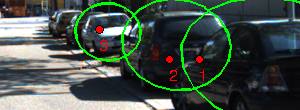
\includegraphics[width=\columnwidth]{results/plotPtransmission_exact_vs_approx_pt_vis-small.png}\\
  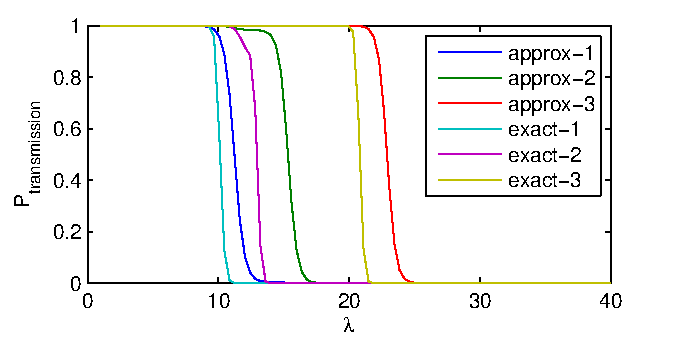
\includegraphics[trim=0.0 0 0.3in 0, clip, width=\columnwidth]{results/plotPtransmission_exact_vs_approx.pdf}
  \caption{Comparing the approximate $\Ptrans$ with exact version. The drop in approximate version of $\Ptrans$ is delayed because we assume drop at the center of the car rather than camera facing face of the car.}
  \label{fig:compare:exact:approx:ptrans}
\end{figure}

Thus, we have modeled the transmission probability to effectively capture the effect of occlusion due to all traffic participants in a scene that lie along a particular ray. We reiterate that our reflection and transmission probabilities are continuous functions, which allows us to define continuous energy functions for association and 3D object localization, as described in the next section.

%\paragraph{Probabilistic occlusion levels}
%With the above modeling and using \eqref{eq:imgform}, 



%% We model the probability of a point $\mathbf{x}_j$ on a object $i$ getting successfully
%% observed in a camera image at point $\trackpj{t}$ is dependent up two factors,
%% (1) reflection and (2) transmission through intermediate space. The reflection
%% part ensures that there is an object to reflect a point at a certain region in
%% the 3D space while transmission part models occlusion.
%% \begin{align}
%%   P^{(ij)}_{\text{observation}} = P^{(ij)}_{\text{reflection}}P^{(j)}_{\text{transmission}}
%% \end{align}

%% %%%%%%%%%%%%%%%%%%%%%%%%%%%%%%%%%%%%%%%%%%%%%%%%%%%%
%% \subsection{Reflection probability}
%% For Lambertian reflection we replace the surface normal with the
%% gradient of occupancy.
%% %
%% \begin{align}
%%   \Prefl = (\max \{0, \nabla \occf^\top
%%   \hat{\mathbf{r}_j}\})^2
%% \end{align}
%% %
%% where $\ray =
%% \frac{K^{-1}\trackpj{t}}{\|K^{-1}\trackpj{t}\|}$ is unit vector in the
%% direction of ray. The gradient in the direction opposite to ray yields -ve
%% probability which needs to be clipped off. Squaring the function keep it
%% smooth near zero.

%% %%%%%%%%%%%%%%%%%%%%%%%%%%%%%%%%%%%%%%%%%%%%%%%%%%%%
%% \subsection{Transmission probability}
%% A model for transmission of light through a material of thickness $x$,
%% density $\rho$ and opacity $k_o$ is given by Beer-Lambert law 
%% %
%% \begin{align}
%%   I(x) = I_0e^{-k_o\rho x}
%% \end{align}
%% %

%% Since both opacity and density are represented by the occupancy function
%% $\occftot = \sum_i \occf$, and also the domain of our $\occftot$ is $[0, 1]$ instead of $[0,
%% \infty]$ as in case of $k_o$; we replace $e^{-k_o\rho}$ by the transparency
%% function $1 - \occftot$. So the transmission probability over a small distance
%% $d\lambda$ is given by
%% %
%% \begin{align}
%%   P_{\text{transmission}}(\lambda + d\lambda) =
%%   P_{\text{transmission}}(\lambda) (1-\occftot)^{d\lambda}
%% \end{align}
%% %

%% For a given 3D point $\mathbf{x}_j = \lambda \ray$, the probability that the
%% point $\trackpj{t}$ is reflected from a distance $\lambda$ is given by

%% \begin{align}
%%   %P^{(j)}_{\text{observation}}(\lambda) &= P_{\text{reflection}}
%%   \Ptrans &=
%%   \prod_{0}^{\lambda} (1 - \occft{\lambda \ray})^{d\lambda} %\\
%%   %= \max \{ 0, (\nabla f_{occ}&(\lambda \ray)^\top \ray) \}
%%   %\prod_{0}^{\lambda} (1 - f_{occ}(\lambda \ray))^{d\lambda}
%%   \label{eq:ptrans-integral}
%% \end{align}
%% where $\prod_{0}^{\lambda}$ represents the \emph{product integral} from $0$ to
%% $\lambda$. 

%% In practice, the integral for transmission probability
%% \eqref{eq:ptrans-integral} is difficult to compute even numerically. So we
%% choose a product of sigmoid function that approximates the behaviour of
%% transmission probability,
%% %
%% \begin{align}
%% \label{eq:evalCumulativePtrans}
%%   \Ptrans &= \prod_i L_u(\trackp{t}; \muiu,\Sigmaiu)L_{\lambda}(\lambda; \mu^i_d)
%% \end{align}
%% %
%% where $L_u(.)$ is sigmoid in image domain with $\mu^i_u$ and $\Sigma^i_u$
%% representing the elliptical projection of $i^{th}$ TP.
%% $L_{\lambda}(.)$ is sigmoid in the depth domain with $\mu^i_d$ as the mean
%% depth of the $i^{th}$ TP.
%% %
%% \begin{align}
%%   L_u(\mathbf{u}; \muiu,\Sigmaiu) &= \frac{1}{
%%     1 + e^{-k_u(1 - (\mathbf{u} - \muiu)^\top\Sigmaiu(\mathbf{u} -
%%     \muiu))}
%%   }
%%   \\
%%   L_{\lambda}(\lambda; \mu^i_d) &= \frac{1}{
%%     1 + e^{-k_d(\lambda - \mu^i_d)}
%% }
%% \end{align}
%% %

%% \begin{comment}%% Comment
%%   A product integral is a simple integral in log domain
%%   \begin{align}
%%     \prod_{0}^{\lambda} (1 - f_{occ}(\lambda \ray))^{d\lambda} =
%%     e^{\int_{1}^{\lambda} \ln{(1 - f_{occ}(\lambda \ray))}{d\lambda}}
%%   \end{align}
%% \end{comment}%% Comment

% \paragraph{Notation}
% We summarize the notation used in the report for quick reference.
% \\
% 
% 
%   \begin{tabular}{|l|l|}
%     \hline
%     Symbol & Meaning \\
%     \hline
%     $\pos{i}{t}$ & Position of $i$th car at time $t$\\
%     $\ori{i}{t}$ & Orientation of $i$th car at time $t$\\
%      $\dimsn{i}$ & 3D bounding box of the car (dimensions)\\
%     $\state{i}{t}$ & State of car $=\{\pos{i}{t}, \ori{i}{t}, \dimsn{i}\}$\\
%     $\egop$ & Position of camera at time $t$\\
%     $\egoo$ & Orientation of camera at time $t$\\
%     $\relp{i}{t}$ & Relative car pose w.r.t. camera \\
%     $\tracklets$ & 3D points tracked on car $i$ in its own frame\\
%     $\trackp{t}$ & Projection of $\tracklets$ in camera\\
%     $\projectionOf{.}$ & Projection function for pose $\relp{i}{t}$\\
%     $\bb{i}$ & 2D bounding box of the car in image\\
%     \hline
%   \end{tabular}
